
% --------------------------------
% 
% --------------------------------

\section{Mexico City Prospective Study (MCPS)}

% --------------------------------
% Recruitment and baseline data
% --------------------------------
\subsection{Recruitment and baseline data}
\begin{frame}
    \frametitle{Recruitment and baseline data}
    \framesubtitle{Overview}

    \begin{columns}

    % Text
    \begin{column}{0.5\textwidth}

        \begin{figure}[htpb]
            \centering
            
\includegraphics[width=1.15\textwidth]{ziyatdinov2023/tapia-conyer2006_header.png}
        \end{figure}

        Over \textbf{\color{complement-1} 150,000} participants were recruited in two districts (figure \ref{fig:mcps-main-map}) between \textbf{\color{complement-2} 1998 and 2004}.

        \begin{itemize}[label=$\bullet$,noitemsep,topsep=5pt]
            \item Baseline questionnaire.
            \item Blood samples.
            \item Physical measurements.
            \item Linkage to mortality.
        \end{itemize}

    \end{column}

    % Image
    \begin{column}{0.5\textwidth}
        \begin{figure}[htpb]
            \centering
            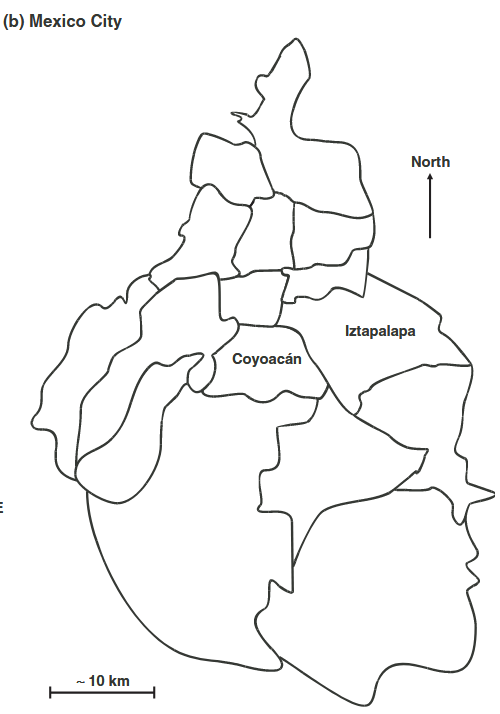
\includegraphics[width=0.45\textwidth]{ziyatdinov2023/map.png}
            \caption{Map showing the location of the MCPS districts \parencite{tapia-conyer-2006}.}
            \label{fig:mcps-main-map}
        \end{figure}
    \end{column}
    \end{columns}
\end{frame}


\begin{frame}
    \frametitle{Recruitment and baseline data}
    \framesubtitle{Baseline data and samples}
    
    \begin{columns}
    % Column 1
    \begin{column}{0.33\textwidth}

        \begin{itemize}[itemsep=2.5pt,topsep=0pt]
            \item \textbf{\color{primary-color} Socio-demographic}
            \begin{itemize}[label=$\bullet$,noitemsep,topsep=1pt]
                {\small\color{complement-text}
                    \item Age and sex
                    \item Area of residence
                    \item Marital status
                    \item Educational achievement
                    \item Occupation
                    \item Income
                    \item Health service provider
                }
            \end{itemize}
            \item \textbf{\color{primary-color} Lifestyle characteristics}
            \begin{itemize}[label=$\bullet$,noitemsep,topsep=1pt]
                {\small\color{complement-text}
                    \item Diet (fruit/vegetables, fried food, types of oil)
                    \item Smoking and alcohol
                    \item Physical activity
                    \item Sleep duration
                }
            \end{itemize}
            \item \textbf{\color{primary-color} Prior diseases and medications}
        \end{itemize}

    \end{column}
    
    % Column 2
    \begin{column}{0.33\textwidth}
        \begin{itemize}[itemsep=2.5pt,topsep=0pt]
            \item \textbf{\color{primary-color} Reproductive history (women)}
            \begin{itemize}[label=$\bullet$,noitemsep,topsep=1pt]
                {\small\color{complement-text}
                    \item Menopausal status
                    \item Hysteroctomy
                    \item Oopheroctomy
                    \item HRT
                    \item Contraceptive use
                    \item Pregnancy (age and number)
                }
            \end{itemize}
            \item \textbf{\color{primary-color} Physical measurements}
            \begin{itemize}[label=$\bullet$,noitemsep,topsep=1pt]
                {\small\color{complement-text}
                    \item Height
                    \item Weight
                    \item Waist and hip circumferece
                    \item Systolic and diastolic blood pressure
                }
            \end{itemize}
        \end{itemize}
    \end{column}

    % Column 3
    \begin{column}{0.33\textwidth}
        \begin{itemize}[itemsep=2.5pt,topsep=0pt]
            \item \textbf{\color{primary-color} Blood samples}
            \begin{itemize}[label=$\bullet$,noitemsep,topsep=1pt]
                {\small\color{complement-text}
                    \item Plasma \& buffy coat
                    \item HbA1c and other essays
                    \item NMR metabolomics
                }
            \end{itemize}
        \end{itemize}
    \end{column}
    
    \end{columns}

\end{frame}

% --------------------------------
% Genetic overview
% --------------------------------
\subsection{Genetic overview}
\begin{frame}
    \frametitle{Genetic overview}
    \framesubtitle{Genetic datasets}

    \begin{columns}
    % Column 1
    \begin{column}{0.5\textwidth}

        Genetic datasets were added later \parencite{ziyatdinov2023}, making it one of the \textbf{\color{complement-1} largest} studies for \textit{non-eurpean} populations.

        \begin{itemize}[itemsep=2pt,topsep=10pt]
            \item<1-> \textbf{\color{primary-color} Genome-Wide Genotyping}
            \begin{itemize}[label=$\bullet$,noitemsep,topsep=0pt]
                \item Illumina - GSAv2 chip array
                \item $n =$ 138,511 individuals
            \end{itemize}
            \item<2-> \textbf{\color{primary-color} Exome Sequencing (WES)}
            \begin{itemize}[label=$\bullet$,noitemsep,topsep=0pt]
                \item $n =$ 141,046 individuals
            \end{itemize}
            \item<3-> \textbf{\color{primary-color} Whole-Genome Sequencing (WGS)}
            \begin{itemize}[label=$\bullet$,noitemsep,topsep=0pt]
                \item $n =$ 9,950 individuals
            \end{itemize}
        \end{itemize}
    \end{column}
    
    % Column 2
    \begin{column}{0.5\textwidth}
        \begin{figure}[htpb]
            \centering
            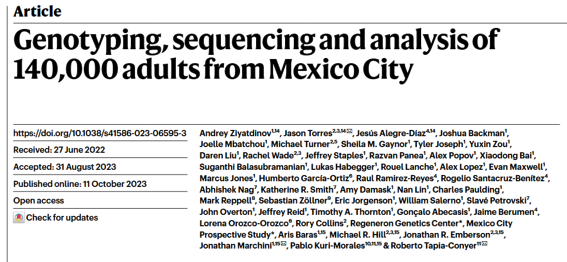
\includegraphics[width=\textwidth]{ziyatdinov2023/ziyatdinov2023_header.png}
        \end{figure}
    \end{column}
    \end{columns}
\end{frame}


% -------------------------
% Methods used
% -------------------------
\subsection{Quality control and other methods}
\begin{frame}
    \frametitle{Quality Control and other methods}
    \framesubtitle{Removing low-quality variants using machine learning}

    \begin{center}
        Using a set of \textcolor{complement-2}{positive} and \textcolor{complement-1}{negative} controls, a \textbf{supervised machine-learning algorithm} was used to discriminate low and high quality variants.
    \end{center}

    \begin{columns}
        % Column 1
        \begin{column}{0.5\textwidth}
            This is a columns.
        \end{column}
        % Column 2
        \begin{column}{0.5\textwidth}
            This is another.
        \end{column}
    \end{columns}
\end{frame}


\begin{frame}
    \frametitle{Quality control and other methods}
    \framesubtitle{Reconstructing pedigree}
    \begin{columns}
        % Column 1
        \begin{column}{0.5\textwidth}
            column
        \end{column}
        % Column 2
        \begin{column}{0.5\textwidth}
            column
        \end{column}
    \end{columns}

\end{frame}

% -------------------------
% Family networks
% -------------------------
\subsection{Family networks}
\begin{frame}
    \frametitle{Family networks}
    \framesubtitle{IBD estimates}

    \begin{columns}
        % Column 1
        \begin{column}{0.5\textwidth}
            At least \textbf{\color{complement-2} 71\% of the population} has a relative present in the dataset.

            \begin{itemize}[label=$\bullet$,noitemsep,topsep=5pt]
                \item \textbf{Parent-offspring:} 31,597 relationships
                \item \textbf{Sibling pairs:} 29,180 relationships
            \end{itemize}

            Close relatedness is explained by families living in \textbf{close proximity}.
        \end{column}

        % Column 2
        \begin{column}{0.5\textwidth}
            \begin{figure}[htpb]
                \centering
                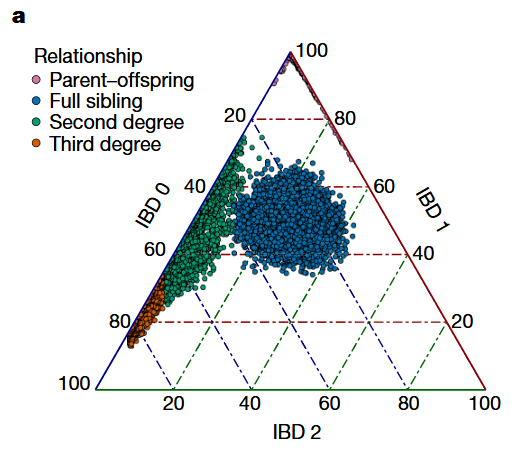
\includegraphics[width=0.85\textwidth]{ziyatdinov2023/familial-relatedness-a.png}
                \caption{Percentage of genome-estimated to have 0 to 3 IBD alleles \parencite{ziyatdinov2023}.}
                \label{fig:percent-genome-ibd}
            \end{figure}
        \end{column}
    \end{columns}

\end{frame}

% Comparison of family networks

\begin{frame}
    \frametitle{Family networks}
    \framesubtitle{Comparison between other dataset}
    \begin{columns}
        % Column 1
        \begin{column}{0.5\textwidth}

            The levels of \textit{relatedness} were
            \begin{itemize}[label=$\bullet$,noitemsep,topsep=5pt]
                \item  much higher than those from the \textcolor{tertiary-color}{UK Biobank (UKB)}.
                \item comparable with the \textcolor{secondary-color}{Geisinger Health Study (GHS)}--both \textcolor{primary-color}{MCPS} and \textcolor{secondary-color}{GHS} recruited in \textit{close proximity}.
            \end{itemize}
        \end{column}
        % Column 2
        \begin{column}{0.5\textwidth}
            \begin{figure}[htpb]
                \centering
                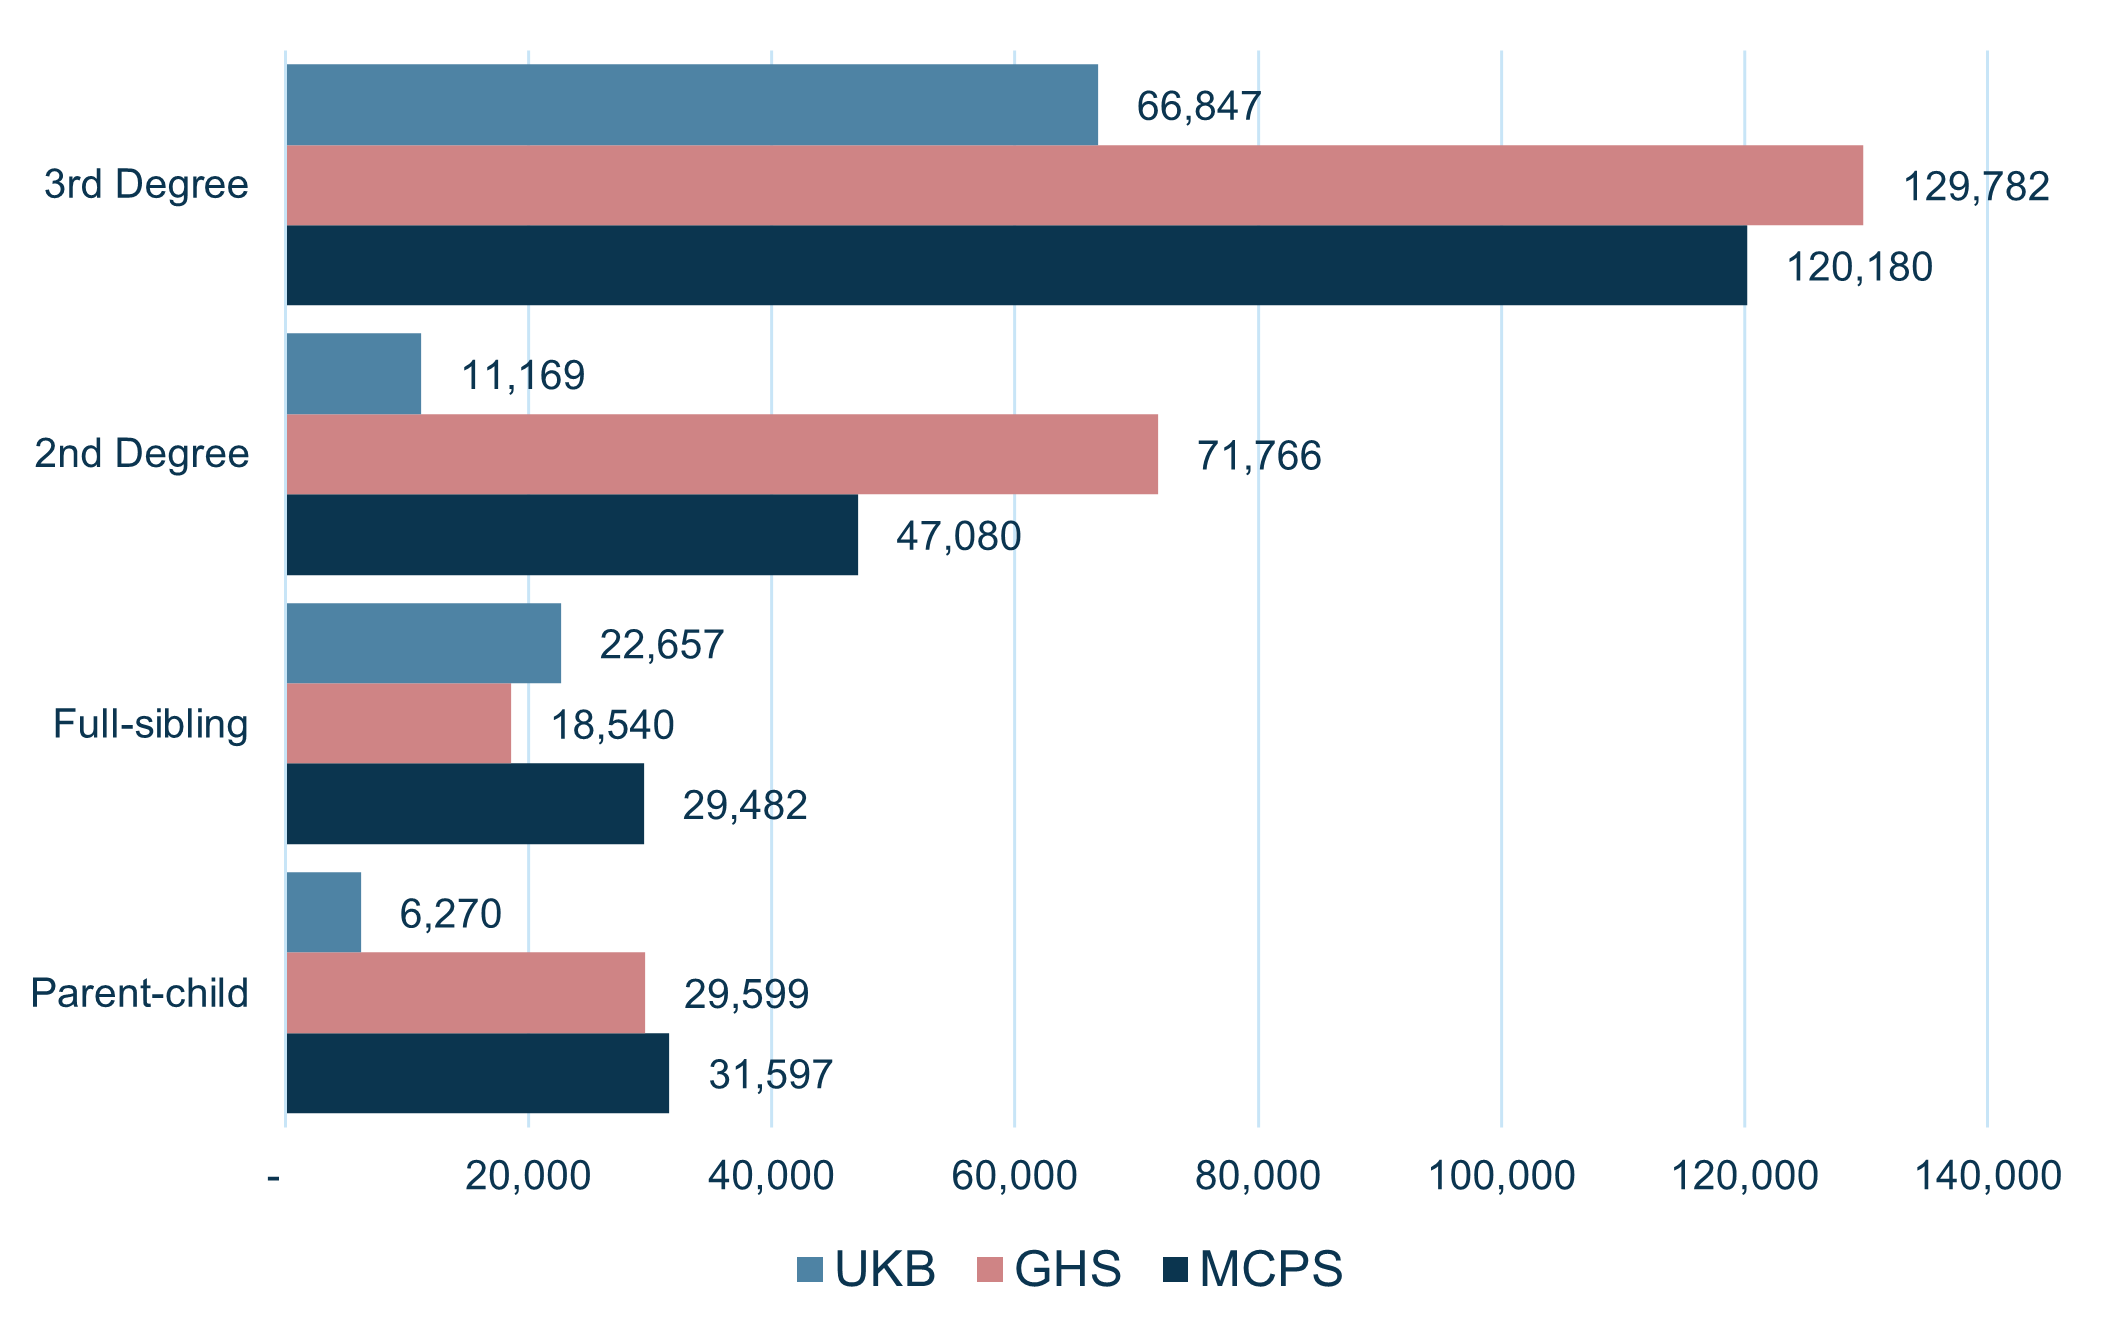
\includegraphics[width=0.95\textwidth]{ziyatdinov2023/dataset-comparison.png}
                \caption{Comparison of network sizes in MCPS, UKB and GHS. Data extracted from Supplementary Table 25 \parencite{ziyatdinov2023}.}
                \label{fig:label}
            \end{figure}
        \end{column}
    \end{columns}
\end{frame}

% -------------------------
% Population structure
% -------------------------
\subsection{Population structure and acestry estimation}
\begin{frame}
    \frametitle{Population structure}
    \framesubtitle{Principal Component Analyses (PCA)}

    \begin{center}
        \textbf{Principal Component Analysis (PCA)} was performed to characteriza heterogeneity and ancestry composition using datasets from:
    \end{center}

    \begin{columns}
        % Column 1
        \begin{column}{0.23\textwidth}
            \begin{itemize}[noitemsep,topsep=5pt]
                \item \textbf{\sffamily\color{primary-color} 1,000 Genomes}
                \begin{itemize}[label=$\bullet$,noitemsep,topsep=0pt]
                {\footnotesize
                    \item African (Yoruba): 107 samples
                    \item European (Iberian): 108 samples
                }
                \end{itemize}
            \end{itemize}
        \end{column}

        % Column 2
        \begin{column}{0.43\textwidth}
            \begin{itemize}[noitemsep,topsep=0pt]
                \item \textbf{\sffamily\color{primary-color} Metabolic Analysis of an Indigenous Sample (MAIS)}
                \begin{itemize}[label=$\bullet$,noitemsep,topsep=5pt]
                {\footnotesize
                    \item Indigenous Mexico (North, Norhwest, Central, South, Southeast): 591 samples
                    \item Data: \textcite{garcia-ortiz2021}
                }
                \end{itemize}
            \end{itemize}
        \end{column}

        % Column 3
        \begin{column}{0.33\textwidth}
            \begin{itemize}[noitemsep,topsep=0pt]
                \item \textbf{\sffamily\color{primary-color} MCPS}
                \begin{itemize}[label=$\bullet$,noitemsep,topsep=5pt]
                {\footnotesize
                    \item Representative: 500 samples
                    \item \textit{Projected: 138,011 samples}
                }
                \end{itemize}
            \end{itemize}
        \end{column}
    \end{columns}
\end{frame}

\begin{frame}
    \frametitle{Population structure}
    \framesubtitle{Principal Component Analyses (PCA)}

    \begin{figure}[htpb]
        \centering
        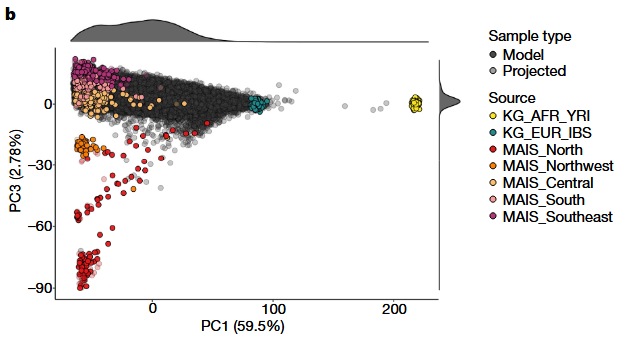
\includegraphics[width=0.95\textwidth]{ziyatdinov2023/pca-analysis.png}
        \caption{PCA analysis to project MCPS data using together Indigenous Mexican, African and European dataset}
        \label{fig:pca}
    \end{figure}

\end{frame}

%\begin{frame}
%    \frametitle{Population structure}
%    \framesubtitle{Principal Components Analyses (PCA)}
%    
%    \begin{columns}
%    % Column 1
%      \begin{column}{0.5\textwidth}
%        To characterize \textit{ancestry composition and heterogeneity}, a PCA analysis was performed using samples relative to pre-Columbian populations:
%
%        \begin{itemize}[noitemsep,topsep=5pt]
%            \item Samples from \href{https://www.internationalgenome.org/data/}{1,000 Genomes} dataset:
%                \begin{itemize}[label=$\bullet$,noitemsep,topsep=2pt]
%                    \item African (KG_AFR_YRI): 108 samples
%                    \item Europan (KG_EUR_IBS): 107 samples
%                \end{itemize}
%        \end{itemize}
%
%      \end{column}
%    % Column 2
%      \begin{column}{0.5\textwidth}
%      \end{column}
%    \end{columns}
%    
%\end{frame}